% !TeX root = ../main.tex

\chapter{Bilder der Umsetzung}\label{chapter:appendix}

	\section{Umsetztung ohne Handposition}
	\begin{figure}[htbp]
		\centering
		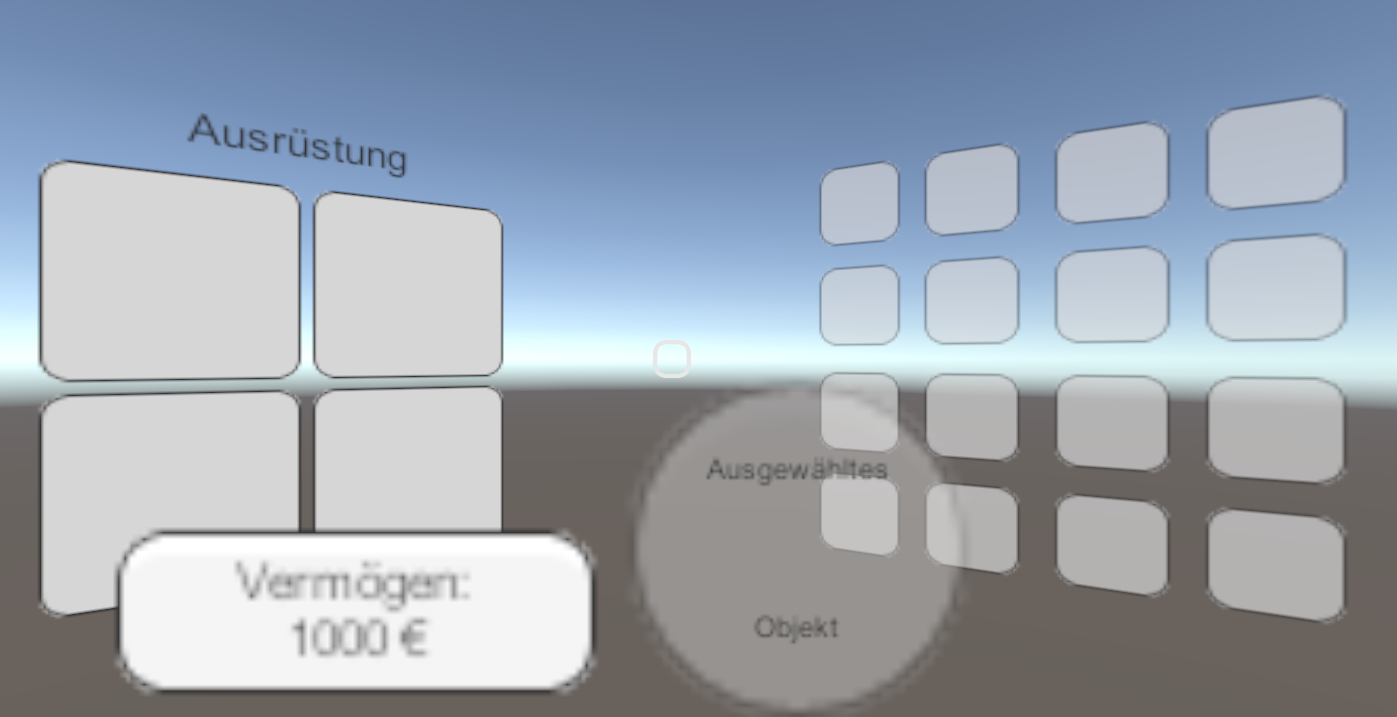
\includegraphics[width=0.75\textwidth]{Fragen/UmsetzungO1.png}
	\end{figure}
	
	\section{Umsetztung mit linker Handposition}
	\begin{figure}[htbp]
		\centering
		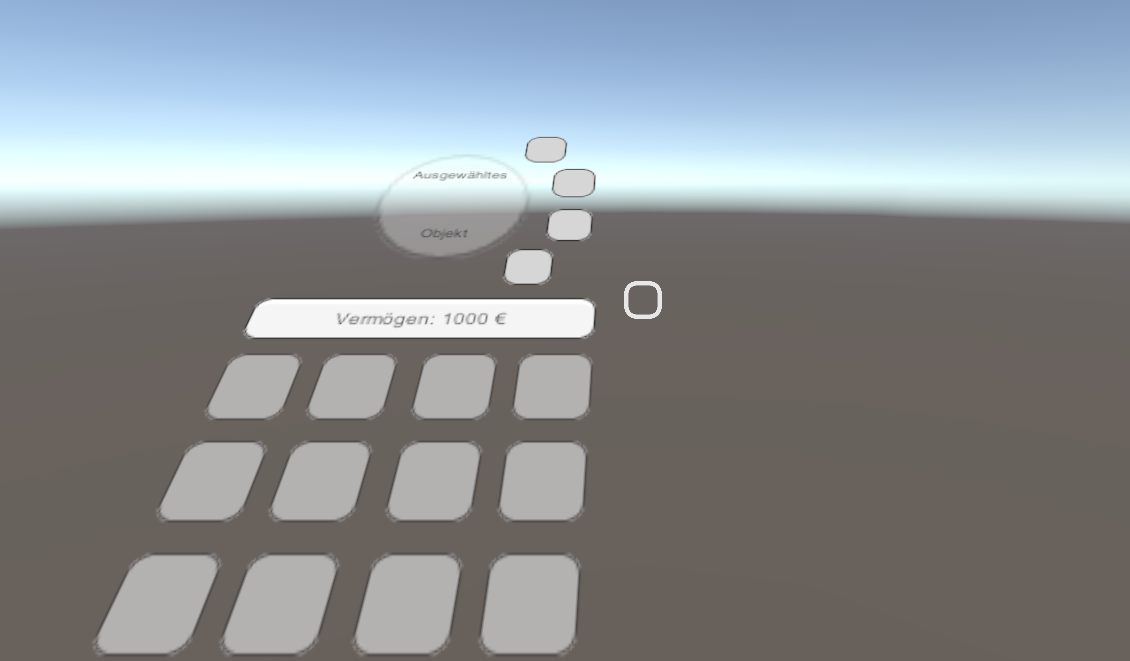
\includegraphics[width=0.7\textwidth]{Fragen/UmsetzungL1.png}
	\end{figure}
	
	\section{Umsetztung mit rechter Handposition - Ausrüstung}
	\begin{figure}[htbp]
		\centering
		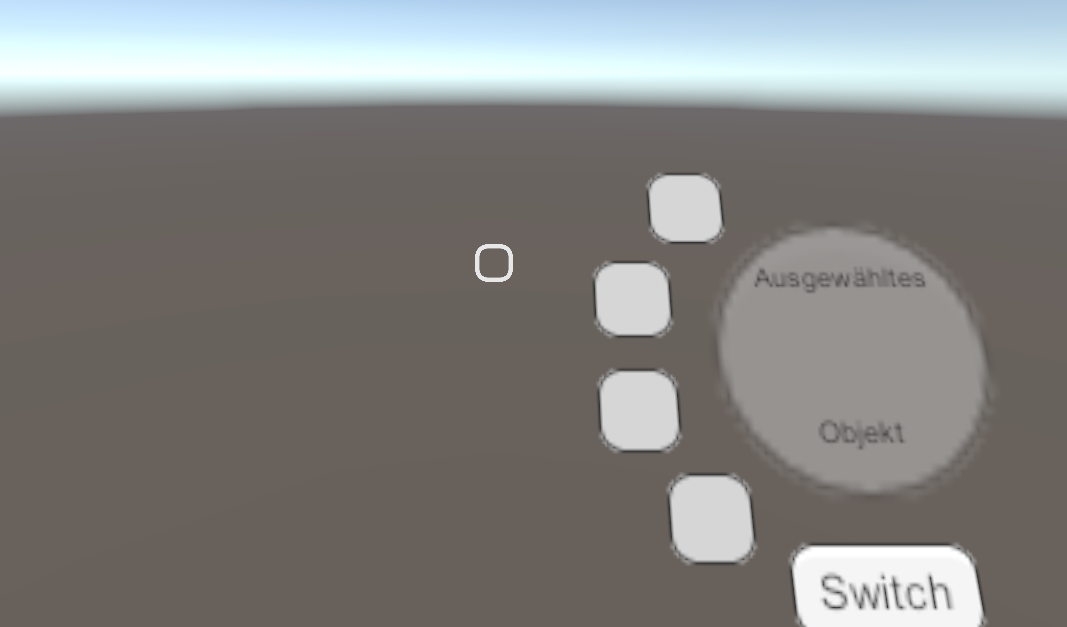
\includegraphics[width=0.75\textwidth]{Fragen/UmsetzungR1.png}
	\end{figure}
	
	\section{Umsetztung mit rechter Handposition - Inventar}
	\begin{figure}[htbp]
		\centering
		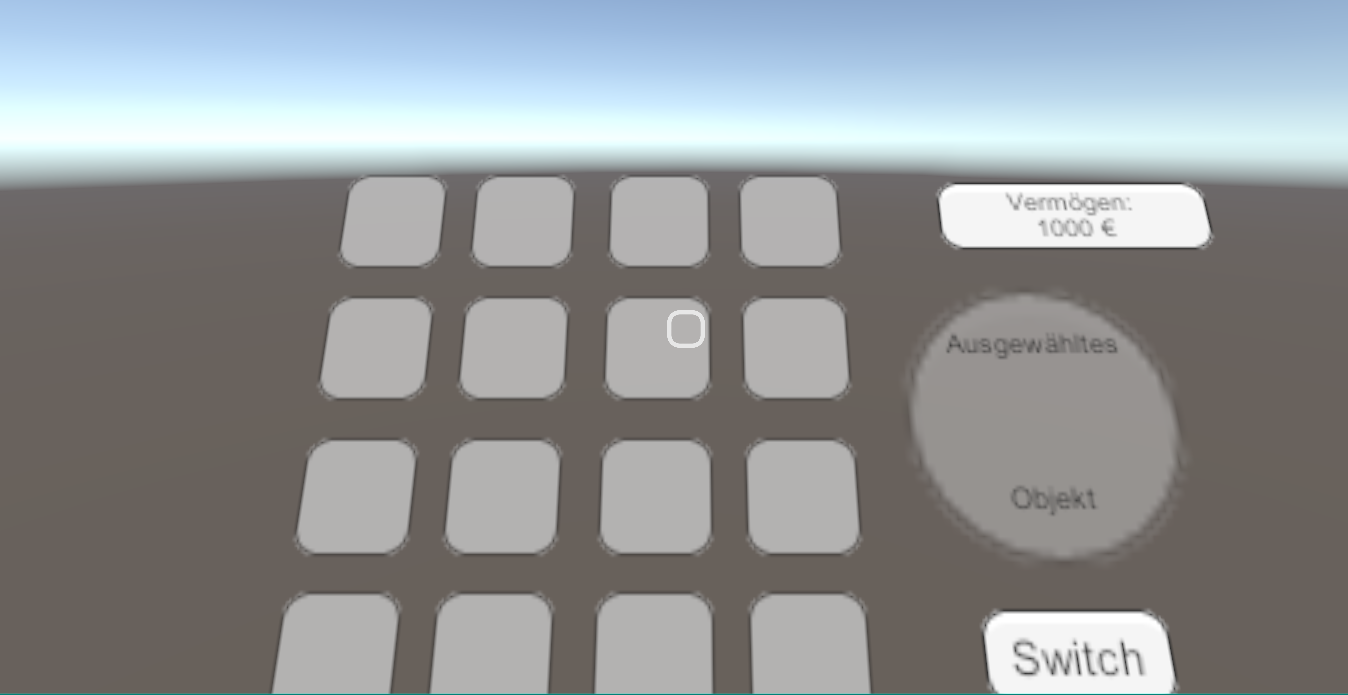
\includegraphics[width=0.75\textwidth]{Fragen/UmsetzungR2.png}
	\end{figure}
	\newpage
	
	\section{Umsetztung mit beiden Handpositionen}
	\begin{figure}[htbp]
		\centering
		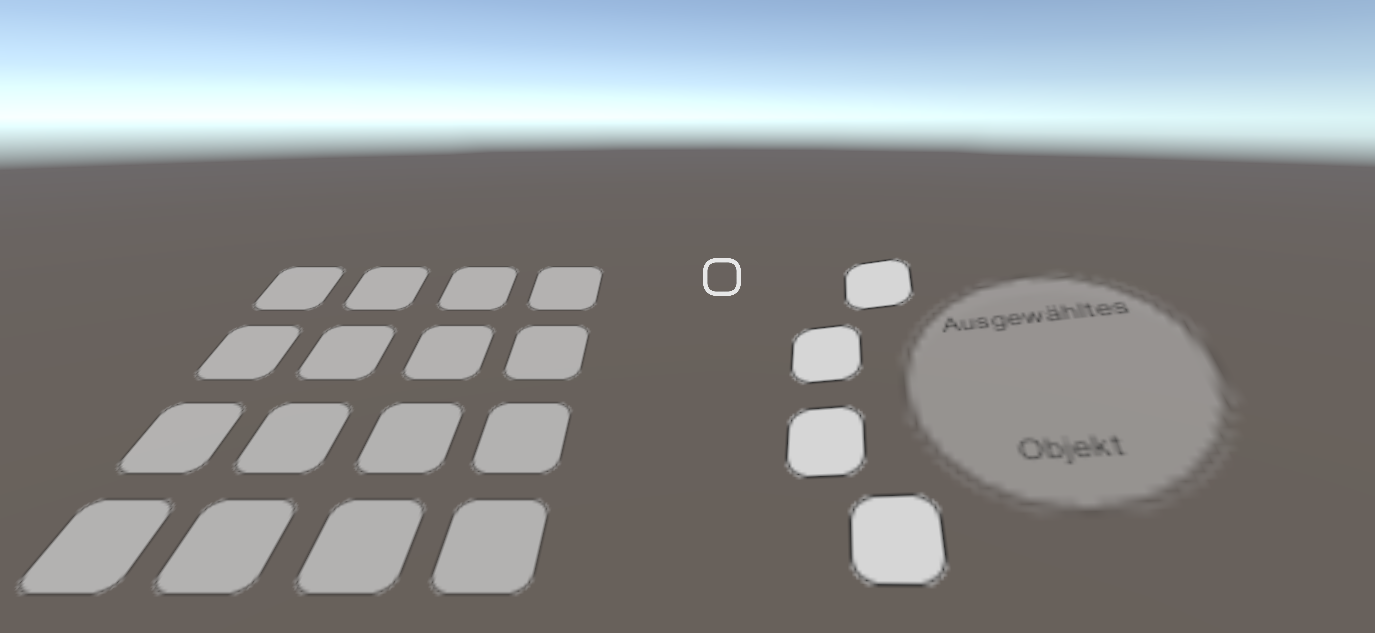
\includegraphics[width=0.75\textwidth]{Fragen/UmsetzungB1.png}
	\end{figure}